% $File: report.tex
% $Date: Fri May 10 23:39:47 2013 +0800
% $Author: wyx <ppwwyyxxc@gmail.com>

\documentclass[11pt,a4paper]{article}

\usepackage{fontspec,amsmath,amssymb,zhspacing,verbatim,minted,listings}
\usepackage{titlesec, titletoc}
\usepackage[hyperfootnotes=false,colorlinks,linkcolor=blue,anchorcolor=blue,citecolor=blue]{hyperref}
\usepackage[sorting=none]{biblatex}
%\usepackage[dvips]{graphicx}
\usepackage{subfigure}
\usepackage{indentfirst}
\usepackage{float}			% don't automatically change location of figure [H]
\usepackage{chngpage}		% use \changetext to change page size
\usepackage{caption}\captionsetup{hypcap=true}  % ref to jump to object instead of caption
\newfontfamily\zhfont[BoldFont=SimHei,ItalicFont=KaiTi_GB2312]{SimSun}
\lstset{keywordstyle=\color{blue!70}, commentstyle=\color{red!50!green!50!blue!50},frame=shadowbox,rulesepcolor=\color{red!20!green!20!blue!20},
basicstyle=\footnotesize\ttfamily}
\zhspacing
\setlength{\parindent}{2em}

%use cell in tabular
\newcommand{\tabincell}[2]{\begin{tabular}{@{}#1@{}}#2\end{tabular}}

%thick shline
\newlength\savewidth
\newcommand\shline{\noalign{\global\savewidth\arrayrulewidth\global\arrayrulewidth 1pt}
                   \hline
                   \noalign{\global\arrayrulewidth\savewidth}}


\renewcommand{\abstractname}{摘要}
\renewcommand{\contentsname}{目录}
\renewcommand{\tablename}{表}
\renewcommand{\figurename}{图}
\defbibheading{bibliography}{\section{References}}
\bibliography{refs.bib}
\newcommand{\figref}[1]{\hyperref[fig:#1]{图\ref*{fig:#1}}}
\newcommand{\secref}[1]{\hyperref[sec:#1]{\ref*{sec:#1}节}}
\newcommand{\tabref}[1]{\hyperref[tab:#1]{表\ref*{tab:#1}}}

% math function
\let\Oldsum\sum
\renewcommand{\sum}{\displaystyle\Oldsum}
\let\Oldprod\prod
\renewcommand{\prod}{\displaystyle\Oldprod}


% $File: mint-defs.tex
% $Date: Fri Jan 06 14:25:30 2012 +0800
% $Author: wyx <ppwwyyxxc@gmail.com>


% \inputmintedConfigured[additional minted options]{lang}{file path}{
\newcommand{\inputmintedConfigured}[3][]{\inputminted[fontsize=\footnotesize,
	label=#3,linenos,frame=lines,framesep=0.8em,tabsize=4,#1]{#2}{#3}}

% \phpsrc[additional minted options]{file path}: show highlighted php source
\newcommand{\phpsrc}[2][]{\inputmintedConfigured[#1]{php}{#2}}
% \phpsrcpart[additional minted options]{file path}{first line}{last line}: show part of highlighted php source
\newcommand{\phpsrcpart}[4][]{\phpsrc[firstline=#3,firstnumber=#3,lastline=#4,#1]{#2}}
% \phpsrceg{example id}
\newcommand{\phpeg}[1]{\inputminted[startinline,
	firstline=2,lastline=2]{php}{res/php-src-eg/#1.php}}

\newcommand{\txtsrc}[2][]{\inputmintedConfigured[#1]{text}{#2}}
\newcommand{\txtsrcpart}[4][]{\txtsrc[firstline=#3,firstnumber=#3,lastline=#4,#1]{#2}}

\newcommand{\pysrc}[2][]{\inputmintedConfigured[#1]{py}{#2}}
\newcommand{\pysrcpart}[4][]{\pysrc[firstline=#3,firstnumber=#3,lastline=#4,#1]{#2}}

\newcommand{\confsrc}[2][]{\inputmintedConfigured[#1]{squidconf}{#2}}
\newcommand{\confsrcpart}[4][]{\confsrc[firstline=#3,firstnumber=#3,lastline=#4,#1]{#2}}

\newcommand{\cppsrc}[2][]{\inputmintedConfigured[#1]{cpp}{#2}}
\newcommand{\cppsrcpart}[4][]{\cppsrc[firstline=#3,firstnumber=#3,lastline=#4,#1]{#2}}


\title{EXAMPLE}
\author{吴育昕\\(清华大学计算机系~北京~100084~ppwwyyxxc@gmail.com)}
\date{January, 2012}

\begin{document}
\changetext{}{2cm}{-1cm}{-1cm}{}
%\fontsize{10pt}{\baselineskip}
%\selectfont
%\maketitle

%\begin{abstract}

	%{\bf 关键词}
%\end{abstract}

% File: title.tex
% Date: Thu Aug 30 16:04:07 2012 +0800
% Author: Yuxin Wu <ppwwyyxxc@gmail.com>

\newcommand{\HUGE}{\fontsize{29pt}{29pt}\selectfont} 
\renewcommand{\today}{\number\year 年 \number\month 月 \number\day 日}
\begin{titlepage} 

% 首行的位置往上调整。但vspace前面需要有东西才会起效。

\phantom{Start!}

\vspace{-1.7cm} 

\begin{flushleft}

\emph{\Large 清华大学计算机系}\\[0.2cm]

\emph{\Large 并行程序设计}\\[4.2cm] 

% Title

%{ \Large \bfseries 程序设计作业一}\\[0.4cm]


{ \Huge \bfseries N-Body Problem}\\[0.4cm]

%{ \Large \bfseries 实现报告} \\[0.4cm]

\end{flushleft}

  

 

\vfill 

 

\begin{flushright}

{

%\setCJKmainfont{Adobe Kaiti Std}

% \pillar:使用一种统一的方法提高行高

\newcommand{\pillar}{ {\Huge \phantom{A}} }

\large

\begin{tabular}{lc}

\pillar 姓名 & 吴育昕\\\cline{2-2}

\pillar 学号 & 2011011271\\\cline{2-2}

\pillar 邮箱 & ppwwyyxxc@gmail.com \\\cline{2-2}

\pillar 时间 & 2012年8月 \\\cline{2-2}

%\pillar 报告日期 & 2012年3月22日 \\\cline{2-2}

\end{tabular}

} 

\end{flushright} 

\end{titlepage} 

\tableofcontents
\titleformat*{\section}{\centering\Large\bf}
% File: intro.tex
% Date: Tue Mar 26 18:42:16 2013 +0800
% Author: Yuxin Wu <ppwwyyxxc@gmail.com>
\section{Introduction}

\begin{enumerate}
	\item 编译:
		程序共有四个版本,分别为串行,MPI,OpenMP,pthread.需通过改变环境变量\verb|DEFINES|分别编译.源码中提供了一个脚本\verb|make_all_version|可以一次性编译出四个可执行文件.
		编译并行版本的环境变量分别为\verb|DEFINES=-DUSE_OMP, -DUSE_MPI, -DUSE_PTH|,单独编译时,可执行文件为\verb|main|
\begin{lstlisting}
$ ./make_all_version
make seq verson ...
done
make omp version ...
done
make pthread version ...
done
make mpi version ...
done
$ DEFINES=-DUSE_OMP make
[dep] main.cc ...
[dep] Gui.cc ...
[dep] Body.cc ...
[dep] utils.cc ...
[dep] common.cc ...
[dep] NBody.cc ...
[dep] NBody_Parallel.cc ...
[cc] NBody_Parallel.cc ...
[cc] NBody.cc ...
[cc] utils.cc ...
[cc] common.cc ...
[cc] Body.cc ...
[cc] Gui.cc ...
[cc] main.cc ...
Linking ...
$
\end{lstlisting}

\item 命令行参数:
	\begin{lstlisting}[basicstyle=\tiny\ttfamily]
$ ./main -h
Usage:
    ./main -b NUM [-r <switch>] [-w <switch>] [-n <NUM_OF_PROC>] [-s <SIZE>] [-t <STEP>] [-h]
Options:
    --ball=NUM,  -b      number of balls. Default: 20.
    --disp=0/1,  -d      a switch on display mode containing a big ball. Default: 1
    --wall=0/1,  -w      a switch on whether to use window border as walls. Default: 1
    --nproc=NUM, -n      number of threads(pthread only). number of CPUs by default
    --size=SIZE, -s      size of window(by pixels). Format: [width]x[height]
                         eg. 1200x800 (default)
    --step=NUM,  -t      number of loops to operate in simulation.
                         NOTE: GUI will be off to calculate time.
    --help,              -h      print help.
\end{lstlisting}
程序支持如下的命令行参数:
\begin{description}
	\item \verb|--ball=NUM|指定小球个数.
	\item \verb|--disp=0/1,--wall=0/1|演示开关与墙壁开关.
	\item \verb|--nproc=NUM|指定pthread使用的线程数量,对其他多线程模式无效.
	\item \verb|--size=SIZE|指定窗口大小.
	\item \verb|--step=NUM|指定循环次数.
	\item \verb|--help|输出帮助信息.
\end{description}

\item 测试运行:
\begin{lstlisting}
$ ./main -b 200 -t 200
0.748785 seconds in total...
$
\end{lstlisting}

\item 界面展示:
\begin{lstlisting}
$ ./main
10.636224 seconds in total...
$ ./main -d 0
14.245977 seconds in total...
\end{lstlisting}

\begin{figure}[H]
	\centering
	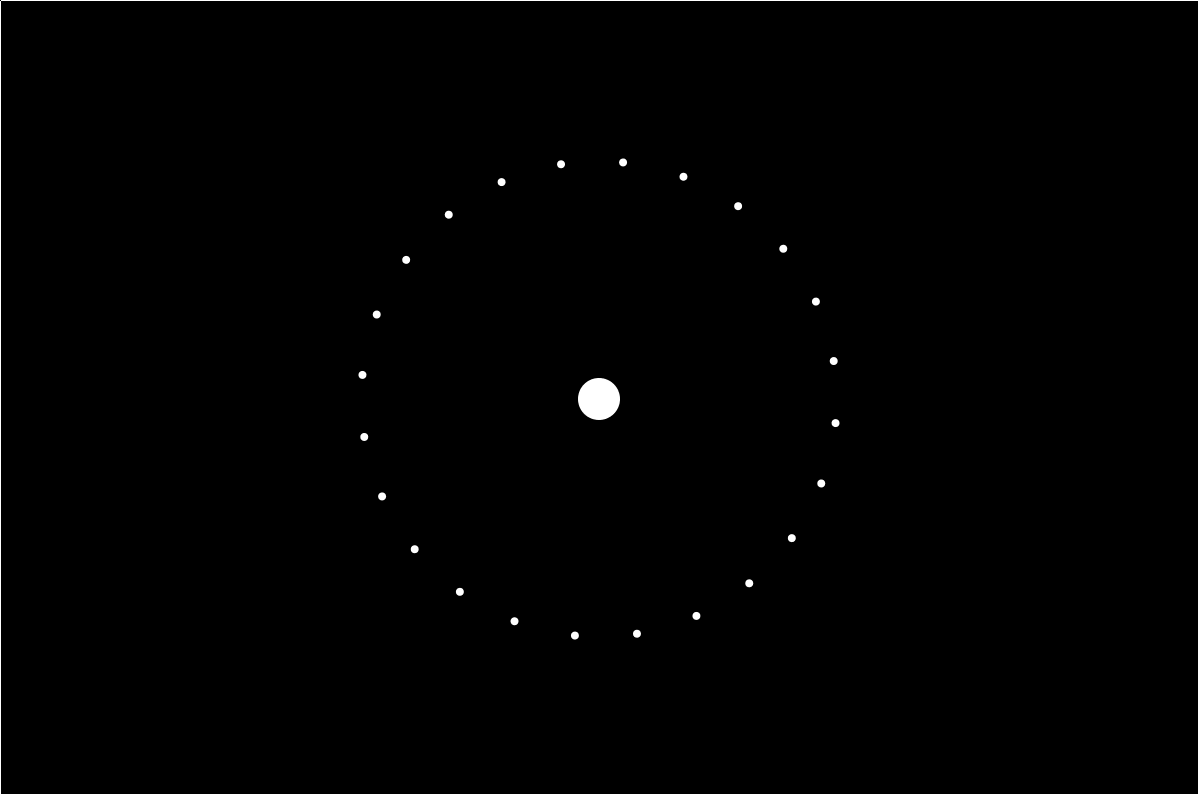
\includegraphics[scale=0.4]{res/screen.png}
	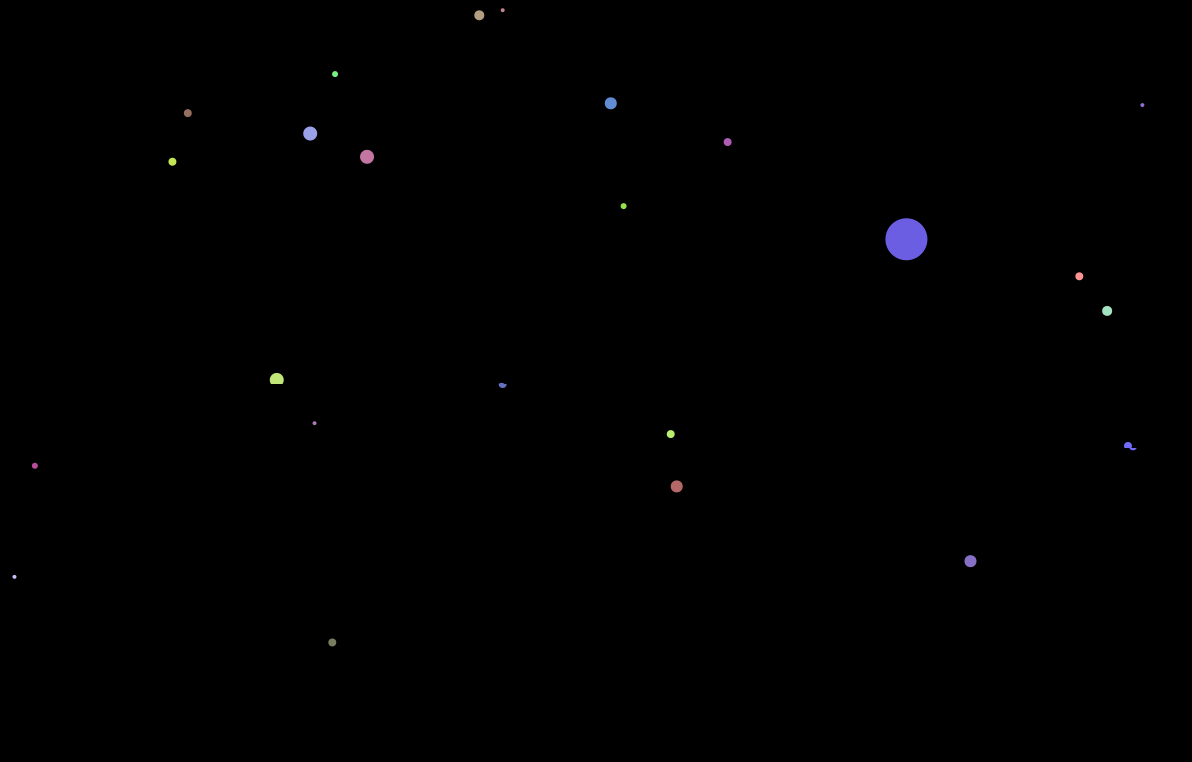
\includegraphics[scale=0.4]{res/screen2.png}
\end{figure}


在窗口中,可使用空格键进行暂停,鼠标左中右键点击屏幕,可查看距点击位置最近的小球信息.按ESC键退出.

\end{enumerate}

% File: theory.tex
% Date: Fri May 10 23:40:38 2013 +0800
% Author: Yuxin Wu <ppwwyyxxc@gmail.com>
\section{Algorithms}
\label{sec:theory}
N体问题\cite{nbody}是在给定一些物体的质量,位置及速度的情形下,计算未来时间中物体如何运动.
本程序是对N体问题的数值模拟,采用纯粹的引力方法\cite{simulation}进行计算.

程序在每次循环中,首先根据牛顿引力公式$ \overrightarrow F_{12} = -\dfrac{GM_1M_2}{|\overrightarrow r_{12}|^2} \dfrac{\overrightarrow r_{12}}{|\overrightarrow r_{12}|}$
分别算出每个物体在这一瞬间的加速度$ \overrightarrow a_t = \sum_{i \ne t}{\dfrac{GM_i \overrightarrow r_{ti}}{|\overrightarrow r_{ti}| ^3} }$,
然后利用$ \Delta \overrightarrow v_t = \overrightarrow a_t$更新各物体的速度.
\cppsrcpart{res/src/Body.cc}{16}{21}

随后,程序判断是否有碰撞发生.判断依据为一个循环的$ dt$时间内是否会有两球的距离小于半径之和,即
$|\overrightarrow r_{ti} +  x\overrightarrow{(v_i - v_t)}| \le R_i + R_t$
是否有 $ 0\le x \le dt$的解.由此找出最先与球$ t$相撞的球,将两球都移动到碰撞点,计算并更新其碰撞后的速度.
\cppsrcpart{res/src/Body.cc}{23}{41}

碰撞时,先将速度分解到碰撞方向与碰撞点的切线方向.
由于碰撞方向上的动量守恒,碰撞点切线方向上的速度不变,再加上能量守恒,可以类似\cite{collision}中的一维情形
列出方程求解.
\cppsrcpart{res/src/Body.cc}{43}{48}

% File: design.tex
% Date: Fri Aug 31 00:50:19 2012 +0800
% Author: Yuxin Wu <ppwwyyxxc@gmail.com>
\section{Design}
	程序通过编译选项\verb|-DUSE_MPI, -DUSE_OMP, -DUSE_PTH|指定使用的多线程库,如果在命令行中选择了\verb|-t|选项,
	则程序直接进入循环计算,完成指定次数的计算后输出时间.
	否则程序会初始化gtk,利用\verb|timeout_signal|方式定时调用计算函数,并在屏幕上输出图像,直至GUI被关闭.

	当定义了\verb|USE_OMP|宏时,程序调用\verb|NBody::omp()|函数进行计算,函数中循环体前有\verb|#pragma omp parallel for schedule(dynamic)|一行,
	对下方的for循环自动进行了动态多线程任务调度.循环体中使用的\verb|NBody::vel_change(), NBody::collision_change()|
	函数分别用于计算引力与碰撞对物体状态造成的改变,被所有多进程模块调用.
	
	当定义了\verb|USE_PTH|宏时,程序调用\verb|NBody::pthread()|函数.
	函数创建\verb|nproc|个线程,每个线程每次领取\verb|pth_unit|个物体的计算任务,并使用变量\verb|int now|用于记录当前未领的任务.
	对每个线程,在需要领取任务时将\verb|now_mutex|锁定,将\verb|now|更新,再解锁.
	引力计算结束后,调用\verb|pthread_barrier_wait|实现同步,再用同样的策略计算碰撞.
	
	当定义了\verb|USE_MPI|宏时,root进程调用\verb|NBody::mpi_master()|函数,其他进程从\verb|main()|中直接调用\verb|NBody::mpi_salve()|
	函数.
	root进程只负责进行任务调度,将任务以\verb|mpi_unit|个为一组发送.
	各进程接收root发送的BEGIN信息以及任务的起始编号,便开始计算,计算完成后向root进程发送FINISH信息及计算数据.
	当引力计算完毕时,root进程发送EXIT信息,随后各进程调用\verb|NBody::share_data()|
	共享root进程的全部数据,然后用同样方法进行碰撞计算.
	随后,如果需要计算墙壁碰撞,则由root进程对所有物体遍历.之后由root进程更新位置并与其他进程广播.




% File: analyse.tex
% Date: Fri Aug 31 01:14:59 2012 +0800
% Author: Yuxin Wu <ppwwyyxxc@gmail.com>
\section{Results and Analysis}


\begin{enumerate}

\item 处理器核数不同时运行时间比较:

\begin{lstlisting}

$ ./pthread -n 2 -b 10000 -t 10                                                                                                                                                                                                                
36.127635 seconds in total...
$ ./pthread -n 4 -b 10000 -t 10                                                                                                                                                                                                                
18.336705 seconds in total...
$ ./pthread -n 6 -b 10000 -t 10                                                                                                                                                                                                                
12.532974 seconds in total...
$ ./pthread -n 8 -b 10000 -t 10                                                                                                                                                                                                                
9.650894 seconds in total...
$ ./pthread -n 10 -b 10000 -t 10
7.912135 seconds in total...
$ ./pthread -n 12 -b 10000 -t 10
6.736707 seconds in total...

$ mpirun -n 2 ./mpi -b 10000 -t 5
36.700927 seconds in total...
$ mpirun -n 4 ./mpi -b 10000 -t 5                                                                                                                                                                                                              
14.856551 seconds in total...
$ mpirun -n 8 ./mpi -b 10000 -t 5                                                                                                                                                                                                              
17.607959 seconds in total...
$ mpirun -n 12 ./mpi -b 10000 -t 5                                                                                                                                                                                                             
13.325384 seconds in total...
\end{lstlisting}
	由以上数据可以得出,pthread与MPI在核数与CPU数相等时效率较高,这与以往的经验吻合.

\item 各并行方式下程序运行时间比较:
\begin{lstlisting}
$ ./pthread -b 10000 -t 10
6.735550 seconds in total...
$ ./omp -b 10000 -t 10                                                                                                                                                                                                                         
20.149873 seconds in total...
$ mpirun -n 12 ./mpi -b 10000 -t 10
26.785754 seconds in total...
$ ./seq -b 10000 -t 10
70.296430 seconds in total...
\end{lstlisting}

本程序的并行效率比较结果表明,pthread效率最高,其次是OpenMP与MPI.这与上一个作业的结果吻合.

\item 球个数不同时运行时间比较:

	\begin{table}[h]
		\centering

		\begin{tabular}{c|c|c|c|c|c|c|c|c}
			\hline
			& 2000	    &5000       &10000      &15000	    &20000	    &30000      &40000			&50000\\\hline
			24  & 7.474266  &15.150455  &17.909214  &23.538911  &32.357338  &58.790446  &94.269225  & 138.547335 \\
			48  & 6.104528  &16.262802  &16.294989  &18.443990  &23.920497  &39.704812  &56.713508  & 79.303986  \\
			60  & 5.965712  &10.075106  &15.898907  &18.610584  &22.252957  &32.892880  &49.755771  & 68.303462  \\
			72  & 4.468587  &10.164223  &15.730339  &19.156377  &20.973644  &30.322637  &43.577078  & 60.674458  \\\hline

		\end{tabular}
		\caption{不同球数,处理器个数下运行时间统计(秒)}
	\end{table}

	\begin{figure}[H]
		\centering
		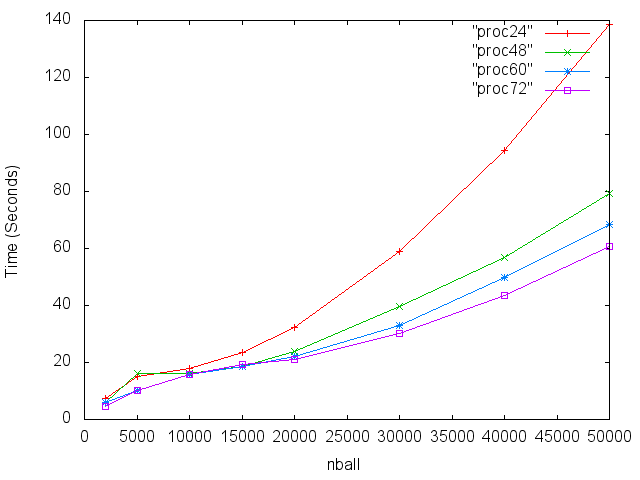
\includegraphics[scale=0.7]{res/ball.png}
	\end{figure}
	可以看出,当核数较少时,时间关于球数大约呈二次函数关系.这与算法$ O(n^2)$的复杂度相吻合.
	核数多时,由于数据量不够大,因此对于球少的情形,并没有显著的加速.


\item 	多核心大数据运行时间比较:

	\begin{figure}[H]
		\centering
		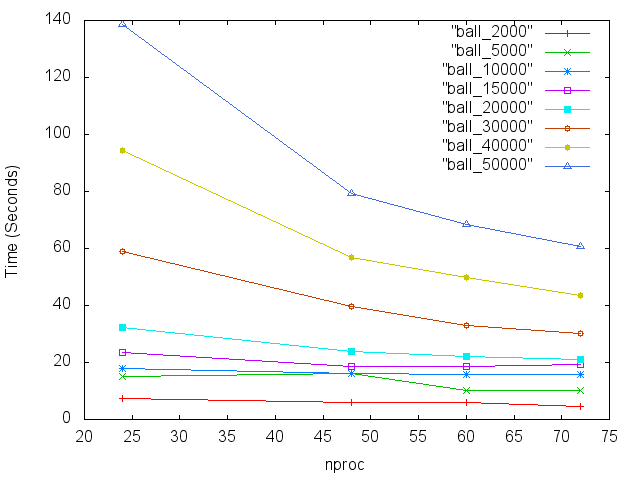
\includegraphics[scale=0.7]{res/proc.png}
	\end{figure}
	可以看出,数据量较小时,多线程的加速效果几乎不可见,这是由于在每个循环周期内,程序会调用两次\verb|NBody::share_data()|来共享计算出的数据,
	每次调用需要广播\verb|MAXN * 4|个\verb|double|,对通信负载非常大.
	但由于题目的特殊性,每次计算都要求获取其余所有物体上一循环结束时的信息,因此这种通信是必不可少的,
	当数据量增大时,多线程的加速效果开始变得明显.

\item 循环次数不同时运行时间比较:
	\begin{figure}[H]
		\centering
		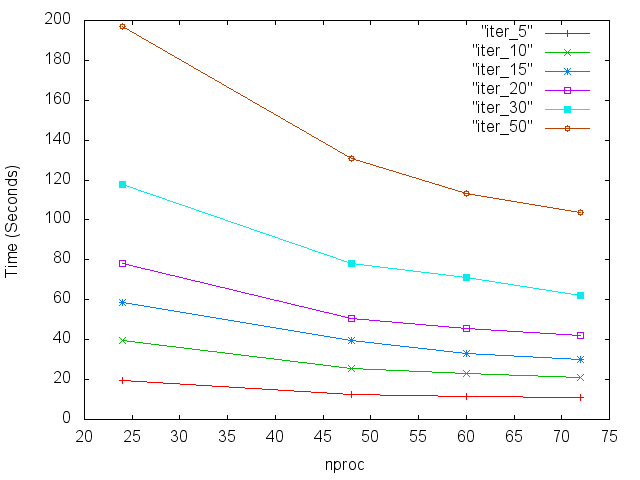
\includegraphics[scale=0.7]{res/iter.png}
	\end{figure}

	从上图中可以看出,循环次数与时间大约成正比.同时还可以发现,循环次数较多时,加速比变得不明显.
	这同样是因为,每次循环结束时,MPI各进程间需要广播数据.

\item 程序效能分析:

	使用gprof,对程序(以pthread版本为例)效能分析部分结果如下:

\begin{lstlisting}[basicstyle=\scriptsize\ttfamily]
$ gprof ./pthread gmon.out 
Flat profile:

Each sample counts as 0.01 seconds.
time   seconds   seconds  calls     name    
40.01     0.34     0.34  4871892    Body::cal_vel(Body const&, double)
31.78     0.61     0.27  4088280    col_time(Body const&, Body const&, double)
9.41      0.69     0.08  5809513    overlap(Body const&, Body const&)
7.06      0.75     0.06  5657909    operator*(double, Vec const&)
5.88      0.80     0.05    15036    NBody::collision_change(int)
3.53      0.83     0.03  4324526    tooclose(Body const&, Body const&)
\end{lstlisting}

	由以上结果,可以看出程序的大部分计算花费在计算引力(\verb|cal_vel()|)与碰撞(\verb|col_time()|,\verb|collision_change()|)上,
	这两个部分包含大量浮点运算. 上表中的\verb|overlap()|与\verb|tooclose()|函数是用于判断物体之间的一些相对位置关系的,
	使用它们使得我的程序展示效果更好,可以看出明显的引力与碰撞效果,没有太多的异常运动,但其中包含的浮点运算(见\secref{theory})消耗了不少资源.
\end{enumerate}

% File: exp.tex
% Date: Fri Aug 31 00:53:05 2012 +0800
% Author: Yuxin Wu <ppwwyyxxc@gmail.com>
\section{Summary \& Experience}
	在第二次作业中,我熟悉了gtkmm的开发,但由于清华FIT楼集群计算机没有gtkmm相关库,在第三次作业中我便使用了Xlib.
	Xlib功能太弱,gtk所支持的信号功能对于这次的程序很重要,因此此次我使用gtk.
	
	在并行方面,由于N体问题每个计算都涉及很多其他数据的参与,
	可以独立并行计算的部分不多,因此对并行算法的设计中不得不在效率与准确度之间做一些取舍.
	因此大家的程序效率,演示效果都有不少差别.如我的MPI程序,就因计算时的几次数据同步耗去了大量时间.

	上次的作业中,算法已经给出,只需设计并行部分.而这次的作业中算法是个难点,较好的选择常数,处理碰撞,
	使得demo中不出现不科学的运动模式花了我大多数的时间.

	这次作业模拟的是物理问题,引力与碰撞的相关问题也让我温习了物理知识,设计常量的过程也让我感受到了宇宙常数的难以选择,不合适的常数总使得物体的运动十分不规则,
	让我更深刻的体会到了关于神秘宇宙常数的``Fine-tuned Universe''的论断\cite{tune}.

\printbibliography

\end{document}

